\documentclass[../main.tex]{subfiles}
\graphicspath{{\subfix{../images/}}}
\begin{document}


\section{Volumes of revolution}
To understand volumes of revolution, we should start by going back to how definite integration works.

Consider a definite integral for a function $f(x)$ that calculates the area between the function and the $x$-axis, between $x=a$ and $x=b$:

\[\int_a^b f(x)\, dx\]

If we look at this graphically, we can see that this area is made up of infinitely small rectangles:

\begin{figure}[h]
    \centering
    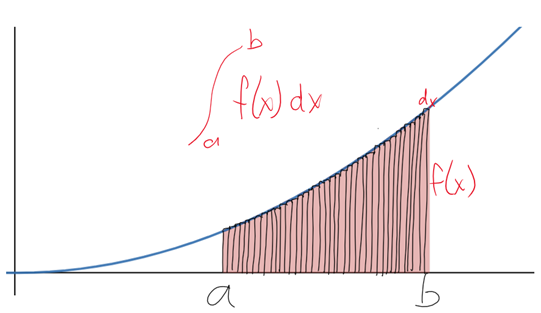
\includegraphics[width=0.5\linewidth]{images/volrev1.png}
\end{figure}

When you consider what the definite integral is saying, the height of each rectangle is $f(x)$, and the width is $dx$. The integral symbol ($\int$) is just an abbreviation of sum, so we are effectively saying find the sum of areas of an infinite number of small rectangles, each of which has area of $f(x)\times dx$.

\subsection*{Disc method}
When we rotate a function about an axis, we can calculate the volume of the shape formed. Visualising the rotation below (this one is about the $x$-axis).

\begin{figure}[h]
    \centering
    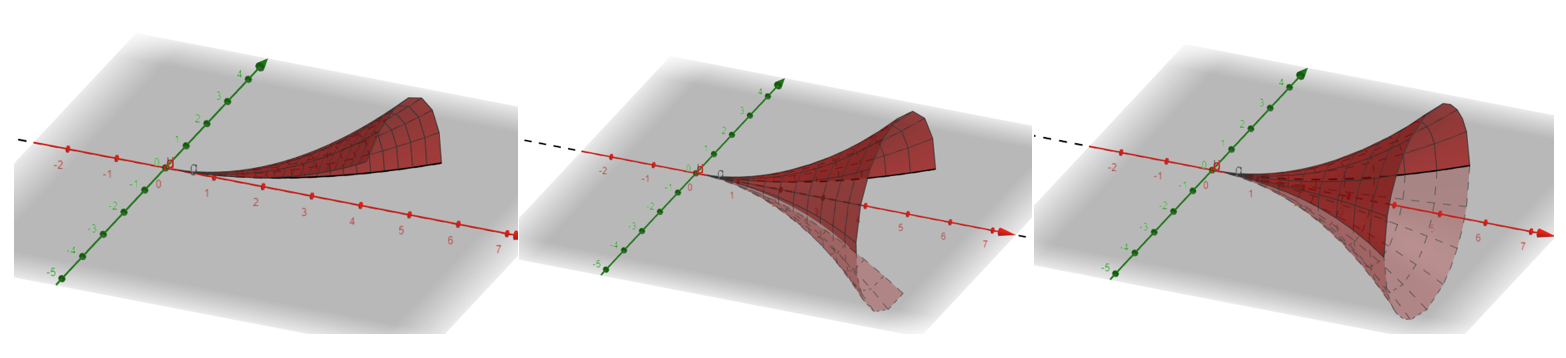
\includegraphics[width=0.75\linewidth]{images/volrev2.png}
\end{figure}

Notice that the rotation is circular, meaning that our 3D shape is made up of an infinite number of infinitely thin circular prisms (cylinders).
    
The volume of a cylinder is $/pi r^2h$. In our case, the radius of each circle is the value of the function, $f(x)$. Again, the height of each cylinder is $dx$. To find the volume we need to do another sum of infinite values, meaning another definite integral.

\begin{figure}[h]
    \centering
    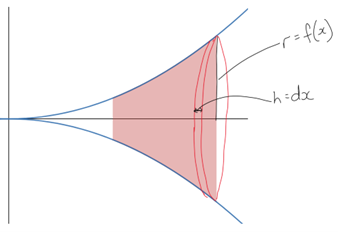
\includegraphics[width=0.5\linewidth]{images/volrev3.png}
\end{figure}

In this case, our sum will be $\int_a^b \pi r^2 dx = \int_a^b \pi (f(x))^2\,dx = \pi \int_a^b (f(x))^2\,dx$

If the rotation is around the $y$-axis, we can simply rearrange the equation so that $x$ is the subject.

i.e. $\int_a^b \pi (f(y))^2\,dy$

\subsection*{Example}
Find the volume of the solid generated by revolving the region bounded by $y=0.1x^2$ and the $x$-axis between $x=2$ and $x=4$ around the $x$-axis.

\begin{figure}[h]
    \centering
    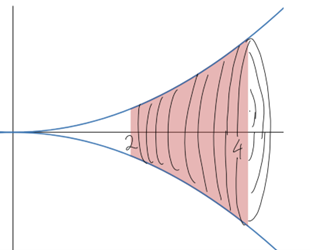
\includegraphics[width=0.5\linewidth]{images/volrev4.png}
\end{figure}

$V=\pi \int_2^4 (0.1x^2)^2\,dx = \pi \int_2^4 0.01x^4\,dx$

$V=\pi[0.002x^5]_2^4=6.23$

\subsection*{Washer method}
If the area between two functions is rotated around an axis, we use the washer method to find the volume. (A washer is just a disc with a hole in the centre of it.)

\begin{figure}[h]
    \centering
    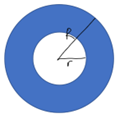
\includegraphics{images/volrev5.png}
\end{figure}

The area of a washer with outer radius of $R$ and inner radius of $r$ is $\pi R^2-\pi r^2=\pi(R^2 - r^2)$

Therefore, the volume of an infinite number of tiny washers between $x=a$ and $x=b$ will be:

$V=\int_a^b \pi (R^2 - r^2)\,dx$

\begin{figure}[h]
    \centering
    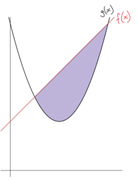
\includegraphics{images/volrev6.png}
\end{figure}

If the outer function is $f(x)$ and the inner function is $g(x)$, then the volume will be:

$\pi \int_a^b (f(x))^2 - (g(x))^2\,dx$
\pagebreak
\subsection*{Example}
Calculate the volume of the solid generated by revolving the area bounded by:
 $y=x+4$ and $y=x^2+2$ about the x-axis.

You will need to find the points of intersection to get the upper and lower limits of the definite integral.

$x^2+2=x+4\\
x^2-x-2=0\\
x=-1, 2$

\begin{figure}[h!]
    \centering
    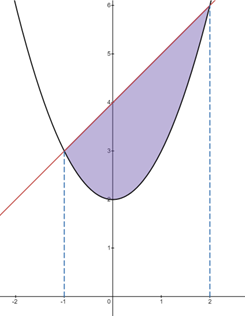
\includegraphics{images/volrev7.png}
\end{figure}

$V=\pi \int_{-1}^2 (x+4)^2 - (x^2+2)^2\,dx$

$V=\pi \int_{-1}^2 (x^2+8x+16) - (x^4+4x^2+4)\,dx$

$V=\pi \int_{-1}^2 (-x^4-4x^2+8x+12)\,dx$

$V=\pi \Bigl[-\frac{x^5}{5}-\frac{4x^3}{3}+4x+12x\Bigr]_{-1}^2$

$V=\pi \Bigl[\frac{128}{5}-\frac{-34}{5} \Bigr]=\frac{162\pi}{5}$

\subsection*{Different axis of rotation}
When the axis of rotation is different from the $x$ or $y$-axis, we just shift the function across so that the axis of rotation is returned to one of those axes.

For example, if we rotate the function $y=x^2$ about the line $y=1$, we need to move the function down 1 so that the axis of rotation returns to the $x$-axis, so it becomes $y=x^2-1$.

This means our definite integral will look like:

$\pi \int_a^b (x^2-1)^2\,dx$

\pagebreak

\subsection*{Questions}
\label{Volumes of revolution}
\begin{enumerate}[itemsep=0.7cm]
    \item 
    The graph below shows the function $y=\cos{x}$, between $x=0$ and $x=\frac{\pi}{2}$, rotated around the $x$-axis.
    \begin{figure}[h]
        \centering
        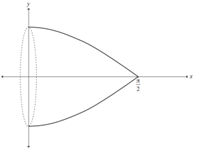
\includegraphics{images/volrev8.png}
    \end{figure}
    Find the volume created by this revolution.

    \item 
    The shaded region below is bounded by the curve $y=x^{\frac{1}{3}}$, the $x$-axis and the line $x=4$.
    \begin{figure}[h]
        \centering
        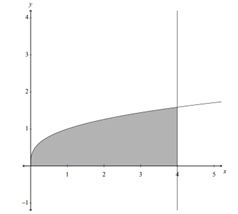
\includegraphics[width=0.3\linewidth]{images/volrev9.png}
    \end{figure}

    Calculate the volume of the solid of revolution generated if this region is rotated around the $x$-axis.

    \item
    The shaded region below is bounded by the curve $y=20-x^2$, the $x$-axis, the $y$-axis and the line $x=4$.
    \begin{figure}[h]
        \centering
        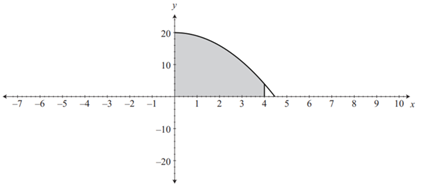
\includegraphics{images/volrev11.png}
    \end{figure}

    Calculate the volume of the solid of revolution generated if this region is rotated around the x-axis.

    \item 
    The shaded region below is bounded by the curve $y=\frac{3}{4}\sqrt{16-x^2}$, the $x$-axis and the $y$-axis.
    \begin{figure}[h]
        \centering
        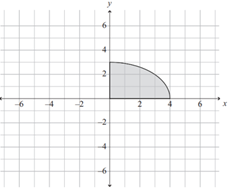
\includegraphics{images/volrev10.png}
    \end{figure}

    Calculate the volume of the solid of revolution generated if this region is rotated around the $y$-axis.

    \item 
    A catering company requires a quantity of plastic disposable cups in which to serve soft drink. They are to be 8cm tall. The designer chooses as a shape the solid or revolution formed by rotating around the x-axis the portion of the curve $y=(x+a)^{\frac{1}{2}}$ between $x=0$ and $x=8$, where a can be varied to give cups different volume.

    \begin{figure}[h]
        \centering
        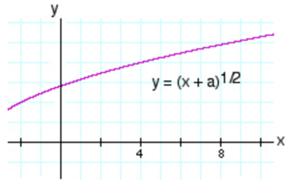
\includegraphics{images/volrev12.png}
    \end{figure}
    \begin{enumerate}
        \item Find the volume of such a cup in general (that is, keeping a in your calculation).
        \item Find the value of a that would give a cup a volume of 200cm3.
    \end{enumerate}
    
    \item 
    Find the volume generated when the area between the curves $y=\ln{x}, y=1$ and $x=\frac{1}{e}$ is rotated about the line $x=\frac{1}{e}$.
    \begin{figure}[h]
        \centering
        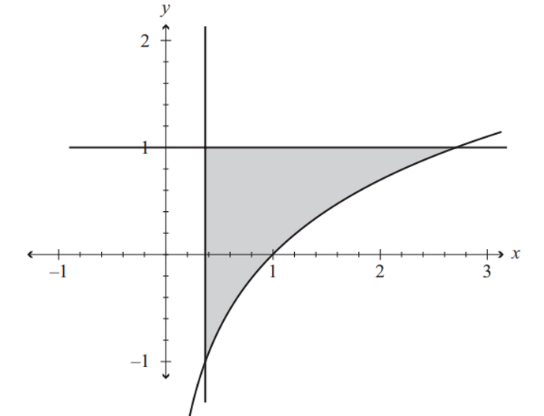
\includegraphics{images/volrev13.png}
    \end{figure}

    \item 
    The shaded region below is bounded by the curve $y=\ln{x}$, the line $x=-1$, the $x$-axis and the line $y$=2.

    \begin{figure}[h]
        \centering
        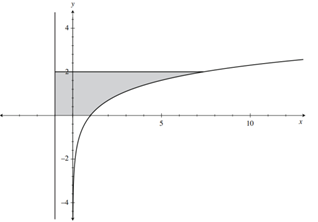
\includegraphics[width=0.3\linewidth]{images/volrev14.png}
    \end{figure}

    Calculate the volume of the solid generated if this region is rotated about the line $x=-1$.

    \item 
    Find the volume generated when the area between $y=\sqrt{x}$ and $y=x$ is rotated around the line $y=-1$

    \begin{figure}[h]
        \centering
        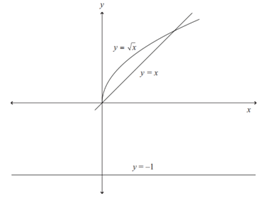
\includegraphics{images/volrev15.png}
    \end{figure}

    \pagebreak
    \item 
    An icemaker produces ice in the shape of paraboloids that may be modelled by rotating the graph of $y^2=4ax$ through 360$^{\circ}$ about the $x$-axis.

    \begin{figure}[h]
        \centering
        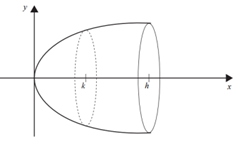
\includegraphics{images/volrev16.png}
    \end{figure}

    Find, in terms of $a$ and $h$, the volume of an ice paraboloid of length $h$.

    \item 
    Prince Rupert’s drops are made by dripping molten glass into cold water. A typical drop is shown in Figure 1.

    \begin{figure}[h]
        \centering
        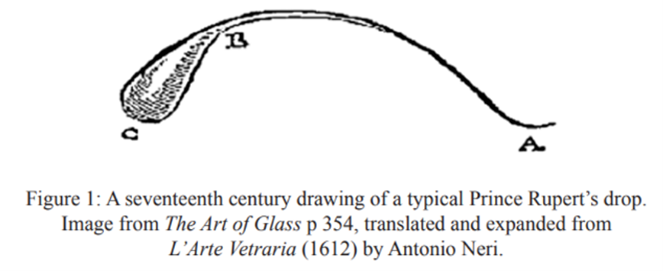
\includegraphics{images/volrev17.png}
    \end{figure}

    A mathematical model for a drop as a volume of revolution uses $y=\sqrt{\phi(e^{-x}-e^{-2x})}$ for $x\geq 0$, and is shown in figure 2, where $\phi$ is the Golden Ratio $\phi=\frac{1+\sqrt{5}}{2}$

    \begin{figure}[h]
        \centering
        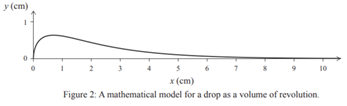
\includegraphics{images/volrev18.png}
    \end{figure}

    \begin{enumerate}
        \item Show that the volume of the drop between $x=0$ and $x=\ln{p}$ is $V=\frac{\pi \phi}{2}(\frac{p-1}{p})^2$.

        \item Hence or otherwise, explain why the volume of the drop is never more than some upper limit $V_L$, no matter how long its tail.
    \end{enumerate}
        
    \pagebreak
    \item 
    Using volumes of revolution, show that the formula for the volume of a truncated right cone (as shown below) is $\frac{1}{3}\pi h(R^2 + Rr + r^2)$.

    You should assume that the top face is parallel to the bottom face.

    \begin{figure}[h]
        \centering
        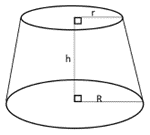
\includegraphics{images/volrev19.png}
    \end{figure}

\end{enumerate}


\pagebreak


\end{document}